In diesem Kapitel werden zunächst die Grundlagen und die Definition des Backends erläutert. In den weiteren Abschnitten dieses Kapitels wird ein Vergleich verschiedener Backend-Frameworks aufgestellt und erläutert wie es zu der Entscheidung für Express.js gekommen ist. Des weiteren wird auf die Implementierung und die verwendeten REST-Schnittstellen eingegangen.

\section{Grundlagen}
\setauthor{Felix Arzt}
Das Backend stellt die funktionelle Schicht in einer IT-Applikation dar. Dies ist der Teil, welcher am nähesten mit dem System verbunden ist und  für die Benutzerin und den Benutzer in den meisten Fällen nicht zugänglich ist, da es den administrativen Bereich darstellt. Dieser ist verantwortlich für die Verarbeitung und Verwaltung von Daten und führt im Hintergrund laufende Vorgänge durch. In dieser Arbeit ist das Backend überwiegend für Datenabfragen und Datensicherungen verantwortlich, aber auch für die Sicherheit in der Anwendung.
\cite{Backend_Basics}

\section{Vergleich von JavaScript Backend-Frameworks}
\setauthor{Felix Arzt}
JavaScript ist immer noch für viele Entwickler: innen überwiegend als Frontend Programmiersprache bekannt. 

"More than 97\% of websites rely on JavaScript, and all major web browser support it"
(vgl. https://blog.hubspot.com/website/java-backend; Zugriff: 26.10.2023)

Dieses Zitat könnte ein Grund dafür sein. Es wurde außerdem nie geplant JavaScript als backend Programmiersprache zu erweitern. Der Hintergedanke bei der Entwicklung von JavaScript, war es eine kompakte script Sprache zu veröffentlichen, um dynamische Web-Erlebnisse zu ermöglichen. Allerdings wurde JS, nicht wie andere Frontend-Webtechnologien, nicht ausschließlich für visuelle Darstellungen entwickelt, sondern wurde als vollwertige Scriptsprache mit erweiterten Funktionen entwickelt. Dies ist mit einer der Gründe, warum JavaScript nun auch als Server-Side-Script Sprache in der IT verwendet wird.
\newline
Der Vorteil eines JavaScript Backends ist, dass man sowohl im Frontend, als auch im Backend, auf eine Sprache setzen kann. Dies ist der Hauptgrund, warum sich unser Projektteam für ein JavaScript basierendes Backend entschieden hat.
\newline
Nachdem nun die Entscheidung für ein JavaScript Backend erläutert wurde, richtet sich nun das Augenmerk auf die zahlreichen verfügbaren Frameworks. In der folgenden Analyse werden die verschiedenen Optionen beleuchtet und ihre spezifischen Eigenschaften sowie ihre Anwendbarkeit im Kontext zu dieser Projektarbeit evaluiert.
\cite{Backend_JavaScript}

\subsection{Nest.js}
\setauthor{Felix Arzt}
\begin{figure}[h]
    \centering
    
\includegraphics[width=0.5\textwidth]{pics/nest_js_logo.jpg}
    \caption{Nest.js Logo}
    \cite{Nest_js_logo}
    \label{fig:mesh1}
\end{figure}

Nest.js ist ein auf NodeJS basierendes Framework, welches Typescript und Vanilla JavaScript unterstützt. 
\newline
"„Vanilla JavaScript“ ist ein Begriff, den Entwickler verwenden, um gewöhnliches JavaScript zu beschreiben. Er definiert die Verwendung der eingebauten JavaScript-Methoden und -Objekte ohne zusätzliche Frameworks oder Bibliotheken."
\newline
(vgl. \url{https://www.yuhiro.de/was-ist-vanilla-javascript/}; Stand 20.02.2024)
\newline
Es kombiniert Elemente von Object Oriented Programming, Functional Programming und Functional Reactive Programming. Im Hintergrund verwendet Nest.js, Express.js als robustes HTTP-Server Framework, dadurch verfügt Nest über eine gewisse Abstraktionsebene.
\cite{Nest_js_Introduction}

\subsubsection{Controllers}
Die Aufgabe eines Controllers besteht darin, requests der Applikation entgegenzunehmen und anschließend eine Response an den Client zurück zu liefern.

\begin{figure}[h]
    \centering
    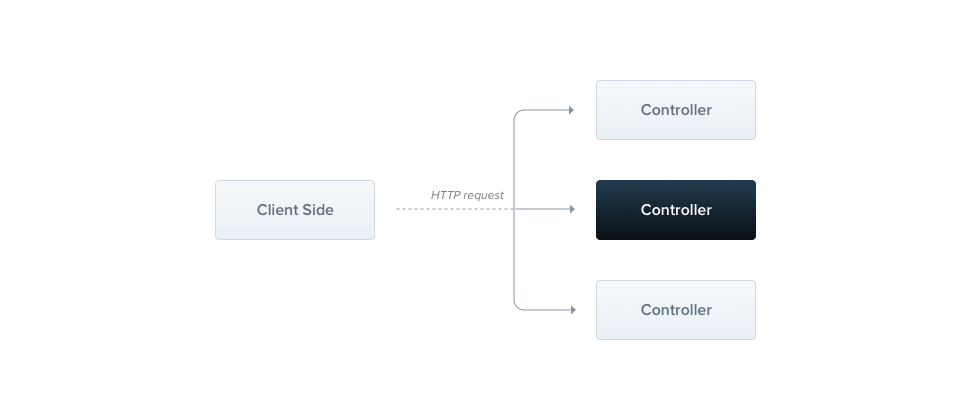
\includegraphics[width=1\textwidth]{pics/Nest_js_Controller.png}
    \caption{Nest.js Controller Architektur}
    \cite{Nest_js_Controller_Architektur}
    \label{fig:mesh1}
\end{figure}

Eingehende Requests werden durch den Routing Mechanismus an den zuständigen Controller weitergeleitet, welcher nun auf den Request reagieren kann und eine dementsprechende Response an den Client sendet. Um einen Controller zu erstellen, werden Klassen und Decorators benötigt. Decorators stellen erforderliche Metadaten, für die jeweiligen Klassen zur Verfügung, dies ermöglicht es Nest, eine Routing-Map zu erstellen, um die Requests an die jeweilig zuständigen Controller weiterzuleiten.
\newline
Der @Controller Decorator ist nötig, um einen neuen Basiscontroller zu erstellen. In diesem Decorator kann man einen Pfad Prefix definieren, um ähnliche Pfade leichter zu gruppieren und dadurch Codeverdoppelungen zu vermeiden. In der Klasse, welche mit dem Controller Decorator definiert wurde, kann man nun folgende HTTP-Methoden erstellen:

\begin{itemize}
    \item Get
    \item Post
    \item Put
    \item Delete
    \item Patch
    \item Options
    \item Head
    \item All
\end{itemize}

\vspace{10mm}

\begin{lstlisting}
import { Controller, Get } from '@nestjs/common';

@Controller('api/users')
export class UsersController {
    @Get(all)
    getAllUsers(): string {
        return 'This function returns all Users';
    }
}
\end{lstlisting}

Der oben gezeigte Beispielcode stellt einen vereinfachten Controller dar, welcher einen GET-Endpoint besitzt. Dieser gibt in folgendem Fall, den oben definierten String zurück.
\cite{Nest_js_Controllers}


\subsubsection{Vorteile}
\begin{itemize}
    \item Leistungsstark
    \newline
    Das Framework wurde so entwickelt, dass sich der Programmierer: in ausschließlich auf das Schreiben des Codes konzentrieren kann. Nest erledigt alle anderen Aspekte, wie zum Beispiel das Thema Sicherheit.
    \item Syntax
    \newline
    Die Syntax von Nest basiert auf dem Frontend Framework Angular, was es für Neulinge einfacher macht, sich in der Projektstruktur zurecht zu finden.
    \item Dokumentation
    \newline
    Die Dokumentation von Nest ist sehr detailliert und leicht zu verstehen.
    \item Typescript
    \newline
    Durch die Kompatibilität mit Typescript, verringert es die Fehleranfälligkeit des Codes, da man im Typescript Kompiliefehler und Warnungen angezeigt bekommt.
\end{itemize}

\subsubsection{Nachteile}
\begin{itemize}
    \item Kompliziert für Anfänger
    \newline
    Für Entwickler: innen die nicht mit Angular vertraut sind, kann das Erlernen von Nest durchaus Schwierigkeiten mit sich bringen.
    \item Kein Know-How in Unternehmen
    \newline
    In Bezug auf diese Projektarbeit, ist einer der größten Nachteile für das Team, dass im Kooperationsunternehmen kein Know-How für Nest.js vorhanden ist, da dieses mit Express.js arbeitet.
\end{itemize}
\cite{Nest_js_Pros_Cons}


\subsection{Express.js}
\setauthor{Felix Arzt}
\begin{figure}[h!]
    \centering
    
\includegraphics[width=0.8\linewidth]{pics/express_logo.png}
    \caption{Express.js Logo}
    \label{fig:enter-label}
\end{figure}
Express.js ist ein Node.js-Framework, das erstmals im November 2010 veröffentlicht wurde. Trotz seiner minimalistischen Ausrichtung zeichnet sich Express durch seine Erweiterbarkeit und Vielseitigkeit aus. Dies wird durch eine Fülle von Libraries und Modules ermöglicht, die in das Framework integriert sind oder von der Entwicklergemeinschaft entwickelt wurden. Diese Ressourcen erleichtern die Bewältigung komplexer Aufgaben, wie die Handhabung von Cookies, Sitzungsverwaltung, Benutzeranmeldung und viele weitere Funktionen, die für moderne Webanwendungen von entscheidender Bedeutung sind.
\newline
Eine der architektonischen Merkmale von Express ist sein Middleware-Konzept. Dieses ermöglicht die Verarbeitung von HTTP-Anfragen in Schichten. Jede Middleware-Funktion kann spezifische Aufgaben übernehmen und ist in der Lage, Requests und Responses zu modifizieren oder zu ergänzen, bevor sie an die nächste Middleware-Funktion weitergeleitet werden. Dies bietet eine hohe Flexibilität und Kontrolle über den Anfragen- und Antwortfluss in einer Express-Anwendung.
\cite{Express_js_Introduction}

\subsubsection{Routing}
Das Routing, im Kontext von Webanwendungen, spielt eine entscheidende Rolle bei der Bestimmung, wie die Anwendung auf eine Clientanfrage in Bezug auf einen spezifischen Endpoint reagiert. Dieser Prozess ist von essenzieller Bedeutung, um Anfragen an die korrekte Ressource oder den gewünschten Endpunkt innerhalb der Anwendung zu leiten. Um diesen Zweck zu erfüllen, sind zwei entscheidende Informationen erforderlich: der Pfad und die HTTP-Methode.
\newline
Der Pfad definiert die URL-Struktur, anhand derer die Anfrage geroutet wird. Dies ermöglicht die Identifikation des gewünschten Endpunkts oder der Ressource innerhalb der Anwendung. Die HTTP-Methode gibt an, welche Aktion auf dem spezifizierten Pfad ausgeführt werden soll. Es ist wichtig anzumerken, dass eine Route innerhalb einer Webanwendung mehrere HTTP-Funktionen besitzen kann. Dies bedeutet, dass eine bestimmte URL-Ressource oder ein Endpoint für verschiedene HTTP-Anfragen unterschiedliche Reaktionen bieten kann. Dies ermöglicht die Implementierung von CRUD-Operationen (Create, Read, Update, Delete) für bestimmte Ressourcen und bietet somit eine flexible und mächtige Möglichkeit zur Interaktion mit der Anwendung.
\cite{Express_js_basic_routing}
\cite{Express_js_routing}

\subsubsection{Middleware}
Middleware Funktionen haben Zugriff auf das Request-Object (\textbf{req}), das Response-Object (\textbf{res}) und auf die \textbf{next} Funktion. Mittels next kann nach Abschluss einer Middleware die nächste Middleware aufgerufen werden, dafür gibt es zwei Möglichkeiten:
\begin{itemize}
    \item ohne Übergabeparameter
        \newline
        Durch das einfache Aufrufen von next ohne Übergabeparameter wird der Request unverändert weitergeleitet und die Ausführung des Codes wird in der nächsten geeigneten Middleware oder Route fortgesetzt. Dieses Vorgehen ermöglicht die nahtlose Verarbeitung von Anfragen und die Kontinuität der Anwendungslogik, ohne den Request zu modifizieren oder zu unterbrechen.
    \item mit Übergabeparameter
        \newline
        In Bezug auf die Übergabeparameter existieren zwei verschiedene Optionen. Die Erste besteht darin, dass, wenn die Zeichenfolge 'route' als Parameter übergeben wird, sämtliche Middleware-Funktionen ignoriert werden, und stattdessen nach einer passenden Route gesucht wird. Die zweite Möglichkeit besteht darin, dass ein anderer Wert als 'route' übergeben wird. Dabei behandelt Express diesen Aufruf als Fehler und überspringt jegliche Middleware- und Route-Funktionen, die keine Fehler zurückgeben. Dieser Ansatz gewährleistet die angemessene Verarbeitung von Anfragen und ermöglicht die gezielte Steuerung des Anwendungsflusses, wobei die Behandlung von Fehlern oder das Überspringen bestimmter Schritte je nach Bedarf erfolgt.
\end{itemize}
\newpage
In einer Express Applikation ist es möglich 5 verschiedene Arten von Middleware einzubinden.

\begin{itemize}
    \item \textbf{Application-Level Middleware}
        \newline
        Diese Middleware wird als Instanz des App-Objekts eingebunden, indem man entweder app.use() oder app.METHOD() benutzt. Bei einer Method Funktion, kann man die drei HTTP-Methoden get, put oder post benutzen. Diese müssen allerdings in Kleinbuchstaben geschrieben werden.
        \newline
        Im folgenden Codebeispiel wird eine Middleware-Funktion implementiert, die bei jedem Request an die App das aktuelle Datum ausgibt. Nachdem das Datum auf der Konsole ausgegeben wird, wird next() aufgerufen, wodurch der Request unverändert bleibt. Falls der Pfad der Syntax "user/:id" entspricht, wird die Ausführung an die erste Middleware weitergeleitet. Wenn die ID den Wert Null aufweist, wird next mit dem Übergabeparameter "route" aufgerufen, der auf die nächste Route verweist. In diesem Fall würde die Middleware "special" als Antwort zurückliefern. Wenn die ID jedoch von null verschieden ist, wird next ohne Übergabeparameter aufgerufen, und der Request wird an die nächste Middleware-Funktion weitergeleitet. In diesem Fall würde die Antwort "regular" lauten.
        \newline
        \begin{lstlisting}[caption=Application-Level Middleware]
            const express = require('express')
            const app = express()

            app.use((req, res, next) => {
                console.log('Time:', Date.now())
                next()
            })
    
            app.get('/user/:id', (req, res, next) => {
                if (req.params.id === '0') next('route')
                else next()
            }, (req, res, next) => {
                res.send('regular')
            })

            app.get('/user/:id', (req, res, next) => {
                res.send('special')
            })
        \end{lstlisting}
    \item \textbf{Router-Level Middleware}
        \newline
        Diese Middleware arbeitet genau gleich wie die Application-Level Middleware, mit dem Unterschied, dass diese eine Instanz des express.Router() ist. Der Nutzen dieser Art von Middleware ist, eine Modularität zu erzeugen, welche es möglich macht, eine Anwendung in kleinere Teile aufzuteilen. Dadurch hat man die Möglichkeit, ein eigenes Untersystem, wie im unten gezeigten Codebeispiel für alle User-Requests zu erstellen. Im folgenden Beispiel werden alle /user Anfragen an den userRouter weitergeleitet und in einem externen File beantwortet.
        \begin{lstlisting}
            const userRouter = require('./userRouter')
            
            app.use('/user', userRouter)
        \end{lstlisting}

        \begin{lstlisting}
            router.get('/getAll', (req, res) => {
                res.send('Alle User')
            }
        \end{lstlisting}
    \item \textbf{Error-Handling Middleware}
        \newline
        Die Error-Handling Middleware funktioniert auf die gleiche Weise wie die oben genannten Middlewares, mit dem kleinen Unterschied, dass 4 Argumente übergeben werden können.
        \begin{lstlisting}[caption=Error-Handling Middleware]
            app.use((err, req, res, next) => {
                console.log(err.stack)
                res.status(500).send('Etwas ist schief gelaufen')
            }
        \end{lstlisting}
    \item \textbf{Built-In Middleware}
        \newline
        Ab Version 4.x verwendet Express nicht mehr Connect und frühere Middleware Funktionen sind in separaten Modulen (third-party middlewares) ausgelagert. Folgende Built-In Middleware-Funktionen sind noch in Express verfügbar:
        \begin{itemize}
            \item \textbf{express.static}
                \newline
                Zur Anzeige von statischem Content, wie zum Beispiel HTML oder Bildern
            \item \textbf{express.json}
                \newline
                Zur Übersetzung von ankommenden JSON requests.
            \item \textbf{express.urlencoded}
                \newline
                Zur Übersetzung von ankommenden URL requests.
        \end{itemize}
    \item \textbf{Third-Party Middleware}
        \newline
        Diese Middleware hat die Aufgabe, einer Express Applikation mehr Funktionalität zu verleihen. Dabei lädt man mittels NPM die gewünschte Middleware aus dem Internet herunter und kann diese anschließend in sein Backend einbauen.
        \begin{lstlisting}[caption=Third-Party Middleware]
            const express = require('express')
            const app = express()
            const cookieParser = require('cookie-parser')

            app.use(cookieParser())
        \end{lstlisting}
        \newpage
        Es gibt folgende Third-Party Middlewares:\newline
        \begin{figure}[h!]
            \centering
            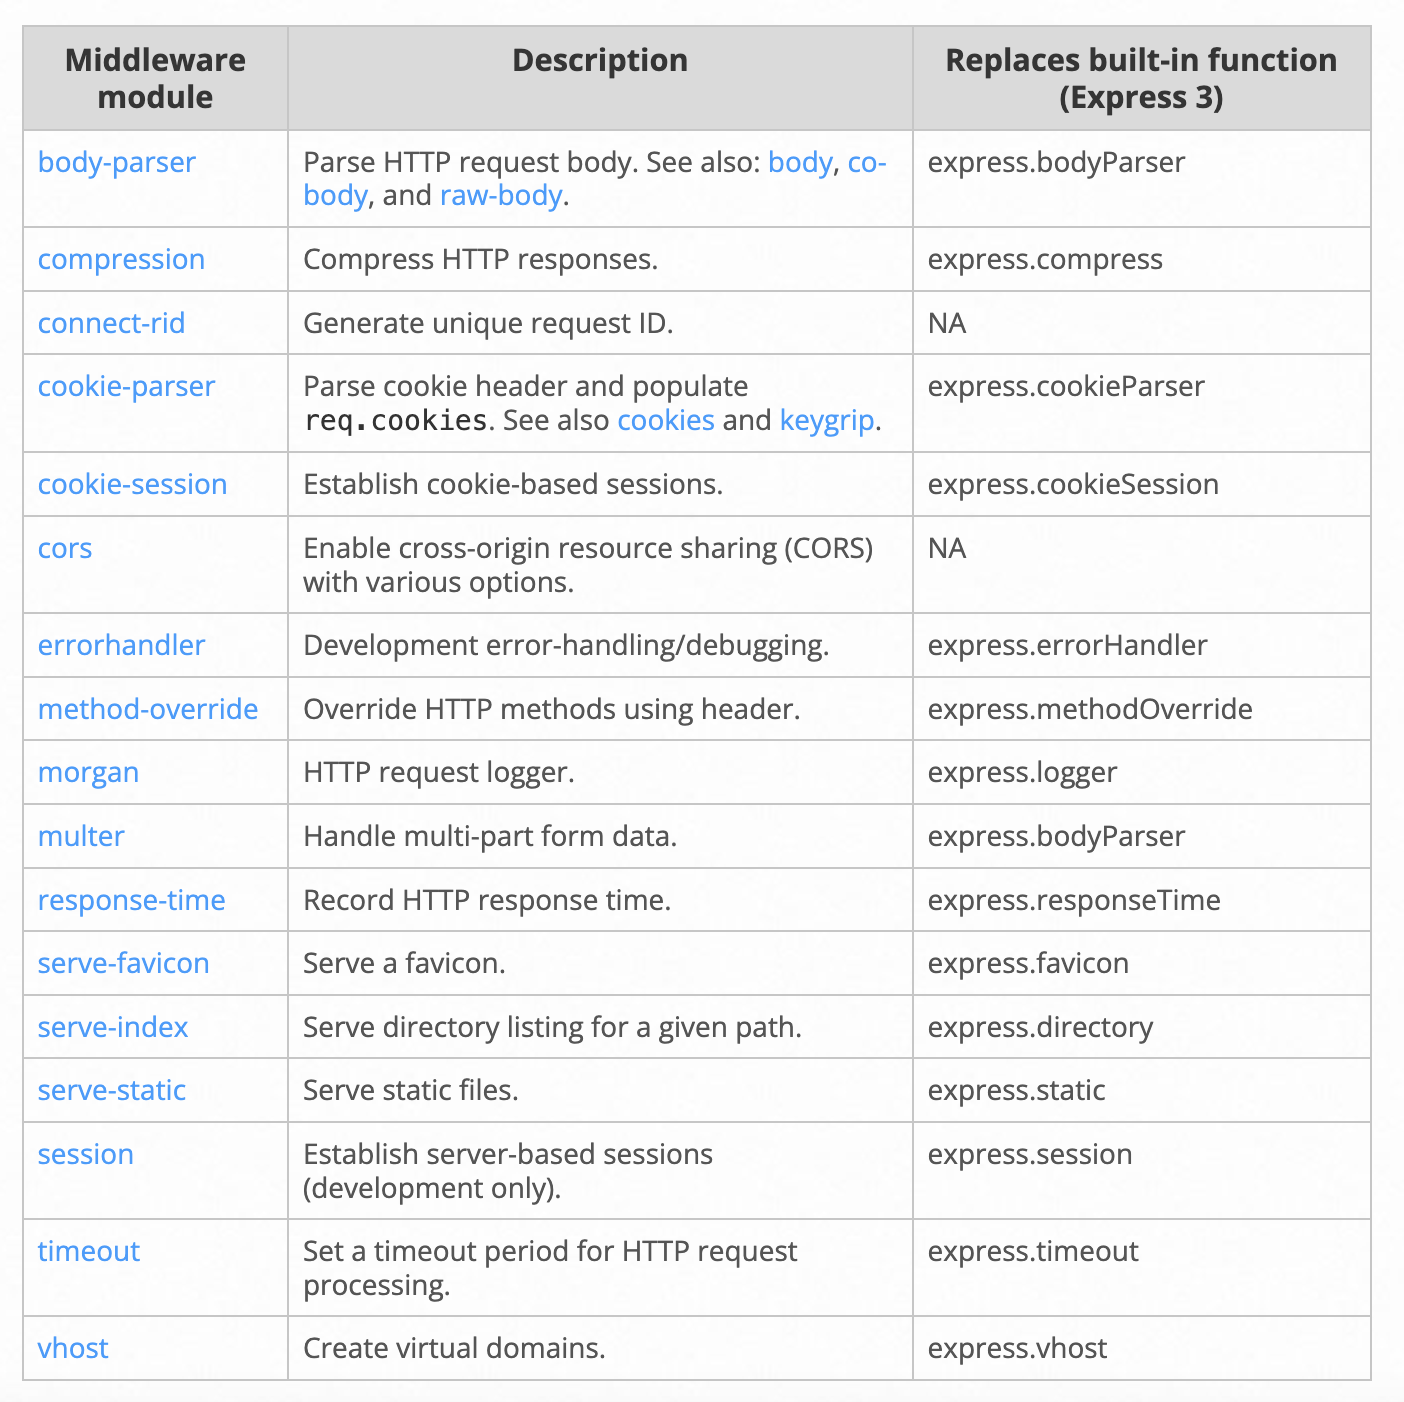
\includegraphics[width=0.8\textwidth]{pics/Third-Party-Middleware.png}
            \caption{Third Party Middlewares}
            \cite{Express_js_third_party_middlewares}
            \label{fig:enter-label}
        \end{figure}
\end{itemize}
\cite{Express_js_writing_middleware}
\cite{Express_js_using_middleware}
\cite{Express_js_middleware_help_1}

\subsubsection{Überschreiben der Express API}
Die Express API besteht aus dem Request und Response Objekt. Diese besitzen verschiedene Funktionen und Übergabeparameter. Man kann die Funktionen der beiden Objekte auf zwei verschiedenen Ebenen verändern. Zum einen kann man diese global, mittels \textbf{express.request} und \textbf{express.response} verändern und zum anderen applikationsspezifisch, durch den Aufruf von \textbf{app.request} und \textbf{app.response}. Eine globale Änderung, wirkt sich auf alle Express-Applikationen im selben Prozess aus, applikationsspezifische Änderungen können erst nach Erstellung einer neuen App durchgeführt werden und gelten dementsprechend nur für das spezifische Objekt. 

\textbf{Überschreiben von Methoden}
\newline
Um die Express API überschreiben zu können, wird an eine bestehende Funktion eine neue, eigens erstellte Methode angehängt.
\begin{lstlisting}[caption=Überschreiben von Methoden]
    app.response.sendStatus = function(statusCode, type, message) {
        return this.contentType(type)
            .status(statusCode)
            .send(message)
    }
\end{lstlisting}
In dem oben gezeigten Fall wurde die sendStatus Funktion überschrieben und es wird von nun an eine eigens erstellte Response zurückgegeben. Die überschriebene Funktion kann nun auf folgende Weise aufgerufen werden.
\begin{lstlisting}
    res.sendStatus(404, 'application/json', '{"error":"resource not found"}            
\end{lstlisting}

\textbf{Überschreiben von Properties}
\newline
Properties in der Express API werden in folgende 2 Kategorien eingeteilt: 
\begin{itemize}
    \item Assigned Properties
    \item Defined as Getters
\end{itemize}
Properties aus Kategorie 1, sind dynamisch zugewiesene Eigenschaften und können daher nicht überschrieben werden. Properties aus der 2. Kategorie können mittels Express API extensions API überschrieben werden. Der folgende Code zeigt, wie man den Wert des \textbf{req.ip} Properties verändern kann. In diesem Fall wird nur die Client-IP aus dem Request-Header ausgegeben.
\begin{lstlisting}
    Object.defineProperty(app.request, 'ip', {
        configurable: true,
        enumerable: true,
        get() { return this.get('Client-IP') }
    }
\end{lstlisting}

\textbf{Überschreiben von Prototypes}
\newline
Um die Express API bereitzustellen, müssen die Request und Response Objekte von derselben Prototypenkette abstammen. Standardmäßig sind \textbf{http.IncomingRequest.prototype} und \textbf{http.ServerResponse.prototype} für die Anfragen und Antworten zuständig. Das Überschreiben der Prototypen sollte, außer wenn es nicht anders möglich ist, nur auf der App-Ebene durchgeführt werden.
\begin{lstlisting}
    Object.setPrototypeOf(Object.getPrototypeOf(app.request), FakeRequest.prototype)
    Object.setPrototypeOf(Object.getPrototypeOf(app.response), FakeResponse.prototype)
\end{lstlisting}
In dem oben gezeigten Beispiel wird der Prototyp von den http.IncomingRequest/ http.ServerResponse auf FakeRequest/FakeResponse umgestellt.
\cite{Express_js_overriding_api}

\subsubsection{Fehlerbehandlung}
Express.js ist mit einer per default definierten Fehlerbehandlung ausgestattet, es ist dementsprechend nicht notwendig eine eigene zu implementieren. In einem Backend ist es essenziell, alle Fehler in der Laufzeit abzufangen, um ein Abstürzen des Servers zu vermeiden. Bei einem nicht asynchronen Code innerhalb einer Middleware oder einer Route, muss man keinen zusätzlichen Arbeitsaufwand investieren, da Express den Fehler von selbst auffängt und anschließend verarbeitet. Bei einem asynchronen Code ist dies anders. In diesem Fall muss next() aufgerufen werden und der Fehler wird in einer anderen Funktion aufgefangen und verarbeitet. Ab der Express Version 5, rufen Middlewares und Routes bei einem asynchronen Code automatisch next() auf, falls ein Fehler auftritt.
\begin{lstlisting}
    app.get('/user/:id', async (req, res, next) => {
        const user = await getUserById(req.params.id)
        res.send(user)
    }
\end{lstlisting}
Im oben gezeigten Beispiel ist die Fehlerbehandlung von Express automatisch implementiert. Falls die Funktion getUserById einen Fehler auswirft, wird automatisch next aufgerufen. Der Übergabeparameter beinhaltet entweder den übergebenen Fehler oder den abgelehnten Wert. Falls keines dieser beiden von der Funktion übergeben wird, wird ein default Fehlerobjekt übergeben.

\textbf{Default Fehlerbehandlung}
\newline
Express stellt eine bereits eingebaute Fehlerbehandlung zur Verfügung, welche sich um jeglichen Fehler in der Applikation kümmert. Diese Fehlerbehandlung muss lediglich am Ende des Middleware-Funktionen-Stacks eingebunden werden. Falls man nun mittels next einen Fehler übergibt, behandelt diese Middleware den Fehler und gibt diesen am Client aus. Tritt ein Fehler auf, werden folgende Informationen im Response Objekt gespeichert:
\begin{itemize}
    \item res.statusCode
        \newline
        Falls dieser Wert außerhalb des 400 und 500 Statuscodebereiches ist, wird automatisch der Fehlercode auf 500 (Server Internal Error) gesetzt.
    \item res.statusMessage
        \newline
        Wird anhand des Fehlercodes gesetzt.
    \item Body
        \newline
        Dies ist der HTML Code der Fehlermessage in einer Produktionsumgebung. Falls dies nicht der Fall ist, heißt das Objekt \textbf{err.stack}.
    \item Header
        \newline
        Alle Header die im \textbf{err.headers} Objekt vorhanden sind.
\end{itemize}
In dem Fall, dass man mittels next einen Fehler aufrufen möchte, man jedoch bereits eine Response an den Client zu schicken begonnen hat, beendet Express die Verbindung und lässt den Request fehlschlagen.

\textbf{Fehlerbehandlung selbst schreiben}
\newline
Wie bereits dargestellt, besteht die Middleware aus 4 Parametern (err, req, res, next). Zu beachten ist, dass die Fehlerbehandlung die letzte implementierte Middleware sein muss. Man kann die Response auf verschiedenste Arten gestalten, zum Beispiel eine HTML-Seite, einen einfachen Fehlertext oder einen JSON-String zurück liefern.
\cite{express_js_error_handling}

\textbf{Debugging}
\newline
Debugging heißt wörtlich übersetzt "Entfernen von Fehlern". Allerdings ist mit Debugging ein mehrstufiger Prozess gemeint, mit dem man einen Fehler identifizieren, die Ursache des Problems herausfinden und anschließend den Fehler beheben beziehungsweise übergehen kann.
\cite{debugging_allgemein}
\newline
Um in Express debuggen zu können und alle internen Ausgaben zu sehen, muss man lediglich die \textbf{DEBUG} Umgebungsvariable auf \textbf{express:*} setzen, wenn man die App startet.
\begin{verbatim}
// Für MacOS
DEBUG=express:* node index.js

// Für Windows
set DEBUG=express:* & node index.js
\end{verbatim}
Man hat nun die Möglichkeit, weitere Optionen für das Debuggen zu definieren.
\begin{center}
    \begin{tabular}{||c c||}
        \hline
        Befehl & Beschreibung \\ [0.5ex] 
        \hline\hline
        DEBUG & Enables/disables specific debugging namespaces \\ 
        \hline
        DEBUG\_COLORS & Whether or not to use colors in the debug output \\
        \hline
        DEBUG\_DEPTH & Object inspection depth \\
        \hline
        DEBUG\_FD & File descriptor to write debug output to \\
        \hline
        DEBUG\_SHOW\_HIDDEN & Shows hidden properties on inspected object \\ [1ex] 
        \hline
    \end{tabular}
\end{center}
\cite{Express_js_third_party_middlewares}

Die Identifizierung von Fehlern und die Debugging-Funktionalität in Visual Studio Code (VS-Code) bieten die Möglichkeit, nicht nur die internen Ausgaben zu erhalten, sondern auch eigens verfasste Funktionen zu überprüfen. Diese Funktionalität wird durch das Setzen von Breakpoints ermöglicht, die einfach neben der Zeilennummer platziert werden. Der Debugger wird daraufhin in der Menüleiste gestartet. Das Starten des Debuggers bewirkt, dass VS-Code die Anwendung ausführt und den Debugger aktiviert. Bei Aufruf der zu überprüfenden Funktion pausiert das Programm an der Stelle, an der zuvor der Breakpoint gesetzt wurde. Hierbei stehen sämtliche existierenden Variablen zur Inspektion zur Verfügung und der Code kann schrittweise durchlaufen werden.
\newline
Eine zusätzliche und oft einfachere Methode, um den eigenen Code zu debuggen, besteht darin, mithilfe von \textbf{console.log} Variablen auszugeben. Auf diese Weise kann überprüft werden, warum der Code fehlerhaft ist und welche Werte in den Variablen enthalten sind.
\cite{express_js_debugging}

\subsection{Express.js vs. Nest.js}
\setauthor{Felix Arzt}
Der bedeutendste Unterschied zwischen den beiden Frameworks besteht darin, dass Express dem Entwickler die Freiheit gewährt, die Art und Weise der Code-Implementierung nach eigenem Ermessen zu gestalten, da keine vordefinierten Regeln vorgeschrieben sind. Im Gegensatz dazu, legt Nest mit seinem Leitprinzip "Konvention vor Konfiguration" besonderen Wert darauf, eine vordefinierte Struktur und klare Konventionen zu etablieren. Dies kann in größeren Entwicklerteams von Vorteil sein, da es dazu beiträgt, einheitliche Regeln und Strukturen zu gewährleisten, denen alle Mitglieder folgen müssen.
\newline
Aufgrund dieser Überlegungen traf das vorliegende Projektteam die Entscheidung, Express.js statt Nest.js zu verwenden. Das Team besteht aus drei Mitgliedern, die in räumlicher Nähe arbeiten und daher in der Lage sind, die Regeln und Strukturen gemeinsam festzulegen, ohne auf vorgegebene Konventionen angewiesen zu sein. Eine weitere maßgebliche Überlegung für die Wahl von Express.js war das bereits vorhandene Know-how im Unternehmen. Alle vorherigen Anwendungen wurden mittels Express.js entwickelt, weshalb letztendlich die Entscheidung für Express.js getroffen wurde.
\cite{express_js_vs_nest_js}

\subsection{Alternativen zu Express.js}
\setauthor{Felix Arzt}
Im Zuge dieser Diplomarbeit standen lediglich die zwei oben genannten Frameworks zur Auswahl, in der Node.js Welt gibt es allerdings noch weitere Frameworks, welche im folgenden Kapitel kurz erläutert werden.

\subsubsection{Hapi.js}
Bei diesem Framework handelt es sich um ein Open-Source Node.js Backend, welches sehr ähnlich zu Express.js ist. Der wohl größte Unterschied zwischen den beiden ist, dass man bei Express.js Middlewares benötigt, um Objekte zu parsen, die allerdings bei Hapi.js nicht benötigt werden. Weitere Unterschiede sind, dass Hapi.js eine konfigurationszentrierte Struktur und vorgefertigte Cache- und Authentifizierungsfunktionen bietet. Bei den integrierten Autorisierungsschemata kann man zwischen Folgenden auswählen:
\begin{itemize}
    \item anonyme Authentifizierung
    \item basisi Authentifizierung
    \item cookie-basiert Authentifizierung
    \item tokenbasiert Authentifizierung
\end{itemize}
Des Weiteren bietet dieses Framework client- und serverseitiges Caching über Catbox.
\newline
\textbf{Vorteile}
\begin{itemize}
    \item Robuste Plugins
    \item Sicheres Framework
        \newline
        Dies wird unter anderem dadurch gewährleistet, indem Fehlermeldungen blockiert werden, welche Daten ausgeben könnten.
    \item Performance
        \newline
        Durch das dauerhafte Cachen wird die Performance der Web-Anwendung verbessert.
    \item Integrierte Authentifizierung
\end{itemize}
\newpage
\textbf{Nachteile}
\begin{itemize}
    \item Kompatibilität
        \newline
        Manche Hapi-Module sind nicht mit anderen Backend-Frameworks, wie zum Beispiel Express.js, kompatibel.
    \item Testen
        \newline
        Das Testen von Endpunkten muss manuell erfolgen, da dieses Framework kaum über Automatisierung verfügt.
\end{itemize}
\cite{backend_hapi}

\subsubsection{Meteor.js}
Meteor.js ist ein "full-stack" JavaScript Plattform, welche zum Entwickeln von Web- und Mobilen-Anwendungen geeignet ist. Das Ziel von Meteor ist, dass sich der Entwickler und die Entwicklerin auf das Erstellen von Funktionalität konzentrieren kann und sich nicht mit Konfigurationen beschäftigen muss. Des Weiteren bietet Meteor ein eigenes Hosting (Galaxy), welches keinerlei Kenntnisse in diesem Bereich benötigt. 
\newline
Beim Erstellen von einer neuen Meteor Applikation, wird standardmäßig ein HTML/JavaScript Frontend und ein Node/MongoDB Backend erstellt. Dies kann man allerdings mit dem Befehl
\begin{verbatim}
    meteor add-platform <platform>
\end{verbatim}
ändern. Kompatible Plattformen in Meteor sind:
\begin{itemize}
    \item React
    \item Vue.js
    \item Svelte
    \item Tailwind CSS
    \item Electron
\end{itemize}
Dies sind nicht alle kompatiblen Plattformen, für eine ausführlichere Auflistung siehe: \url{https://www.meteor.com/}
\newpage
\textbf{Vorteile}
\begin{itemize}
    \item Hohe Kompatibilität mit JavaScript Frontend Frameworks
    \item Full-Stack Framework
    \item Eigenes Hosting
\end{itemize}
\textbf{Nachteile}
\begin{itemize}
    \item Ausschließlich mit MongoDB kompatibel
    \item Full-Stack Framework
\end{itemize}
Full-Stack Framework steht sowohl als Vor- und Nachteil, da dies in manchen Fällen durchaus Sinn ergeben kann, allerdings die Limitation auf gewisse Frameworks in manchen Fällen nicht von Vorteil ist.
\cite{backend_meteor}
\cite{backend_meteor_1}

Es gibt auch außerhalb der Nodes.js Welt Backend-Frameworks, die eine durchaus überlegenswerte Alternative darstellen würde.

\subsubsection{Laravel}
Ist ein PHP basiertes Backend Framework, welches auf dem Symfony Framework aufbaut und daher über einige gut getestete Komponenten verfügt. Des Weiteren kann man über eine eingebaute CLI (command line interface), Code generieren und/oder Tasks aufrufen. Es verfügt ebenfalls über ein eingebautes routing-System und einem ORM (object relational mapping), wodurch man mit der Datenbank mittels PHP-Objekten kommunizieren kann, anstatt SQL-Abfragen zu schreiben.
\newline
\textbf{Vorteile}
\begin{itemize}
    \item Testen
        \newline
        Durch das eingebaute Framework PHPUnit ist das automatische Testen vom Programmcode wesentlich vereinfacht. Mit der Funktion "mocking" ist es möglich unterschiedliche Szenarien zu testen.
    \item Syntax
        \newline
        Bietet eine klare und ausdrucksstarke Syntax, wodurch das Schreiben und Lesen von Code vereinfacht wird.
    \item MVC-Architektur
        \newline
        Nutzt das Model-View-Controller (MVC) Prinzip, wodurch Datenmodell, Präsentationsschicht und Anwendungslogik klar voneinander getrennt sind.
\end{itemize}

\textbf{Nachteile}
\begin{itemize}
    \item Hosting
        \newline
        Laravel benötigt des Öfteren besondere Hosting Anforderungen, welche nicht von allen Anbietern unterstützt werden.
\end{itemize}
\cite{backend_laravel}

\subsubsection{Quarkus}
Ist ein Kubernetes-native Java Framework für die Java Virtual Machines, welches auf dem Dependency-Injection Prinzip aufbaut. Dadurch kann mittels Extensions und Dependencies die Funktionalität so erweitert werden, dass sie für das spezifische Projekt passend ist. Das Framework ist speziell für das Entwickeln von Cloud-nativen Java-Anwendungen optimiert. 

\textbf{Vorteile}
\begin{itemize}
    \item Effizienter Speicherverbrauch
        \newline
        Durch optimierte Laufzeit und die native Kompilierungstechnologie wird der Speicherverbrauch minimiert.
    \item Reaktive Programmierung
        \newline
        Anwendungen können auf asynchrone, nicht-blockierende Weise entwickelt werden, wodurch eine hohe Skalierbarkeit und Leistungsfähigkeit erreicht wird.
\end{itemize}

\textbf{Nachteile}
\begin{itemize}
    \item Konfiguration
        \newline
        Durch die Vielseitigkeit des Frameworks kann die Konfiguration durchaus komplex werden.
\end{itemize}

\section{Implementierung von Express.js}
\setauthor{Felix Arzt}
Da nun die vielseitigen Funktionen von Express.js bekannt sind, geht es nun an die Implementierung des Frameworks. Voraussetzung dafür ist, dass in dem Projektordner bereits der \textbf{Node Package Manager} hinzugefügt worden ist und dadurch auch das \textbf{package.json} File. Diesen kann man ganz einfach mit dem Befehl:
\begin{verbatim}
npm init
\end{verbatim}
hinzufügen. Durch Ausführen dieses Befehls, kann man verschiedenste Einstellungen tätigen, wie zum Beispiel die Version oder den Namen seiner Applikation. Diese Schritte hat unser Projektteam jedoch bis auf einen Übersprungen. Man muss nämlich das sogenannte Hauptfile bestimmen, von welchem aus das Backend gestartet werden kann. In diesem Projekt haben wir dieses File \textbf{server.js} genannt. Wenn dieser Schritt erledigt ist, kann man auch schon Express.js mit folgendem Befehl installieren:
\begin{verbatim}
npm install express
\end{verbatim}
Dadurch wird die neueste, öffentliche Version von Express.js installiert und ins package.json File, mit der verwendeten Version geschrieben. Dies ist dazu da, damit alle anderen Projektmitglieder lediglich mit dem Befehl
\begin{verbatim}
npm install
\end{verbatim}
alle hinzugefügten Modulen nachinstallieren können. Was man allerdings hierbei beachten muss, ist dass bei der Versionsnummer davor Standardmäßig ein \verb|^| gestzt wird. Dieses Zeichen bewirkt ein automatisches updaten der Version, falls eine neuere veröffentlicht worden ist. Da man dies allerdings in den meisten Fällen nicht haben möchte, da dadurch Funktionen auf einmal nicht mehr funktionieren können, hat dieses Projektteam diese Zeichen bei allen installierten Modulen entfernt und nimmt Updates manuell vor.
\newline
\cite{installing_express_js}
\newline
Da nun das Framework Express.js installiert ist, kann man beginnen den einfachst möglichen Server zu erstellen.
\begin{lstlisting}
    const express = require('express')
    const app = express()
    const port = 3000

    app.get('/', (req, res) => {
        res.send('Hello World')
    })

    app.listen(port, () => {
        console.log(`Server is running on port ${port}`)
    })
\end{lstlisting}
Bei diesem Beispiel wird zu Beginn mit dem Befehl \textbf{require()} ein JavaScript File gelesen, ausgeführt und das Return-Objekt zurückgegeben. Anschließend wird dieses Objekt ausgeführt und als neue Variable gespeichert. Mit dieser Variable kann man nun den ersten Endpunkt definieren. In dem obigen Beispiel wird auf der Basis-URL \verb|(/)| Hello World zurück gegeben. Im letzten Schritt, wird der Server auf dem bereits definierten Port gestartet und gibt eine Nachricht auf der Konsole aus. Den Server startet man mit dem Befehl
\begin{verbatim}
node server.js
\end{verbatim}
Voraussetzung dafür ist, dass das File server.js heißt und im \textbf{npm init} Vorgang auch als Hauptfile definiert worden ist.
\newline
\cite{creating_basic_server}

\section{REST API}
\setauthor{Felix Arzt}
Der Begriff REST API steht für "Representational State Transfer - Application Programm Interface" und ermöglicht den Austausch von Informationen, welche sich auf unterschiedlichen Systemen befinden. In diesem Kapitel wird es vorrangig, um die von diesem Team entwickelten Endpunkte des Backends gehen. Grundsätzlich wird in unserer Arbeit zwischen zwei großen, übergeordneten Endpunkten (User und Projekte) unterschieden, bei welchem man anschließend das dazugehörige JSON-Objekt zurück geliefert bekommt. Mit den Übergabeparametern wird im Router-File entschieden, welche Datenbankabfrage gerade aus dem Frontend aufgerufen wurde. Dazu wird der Parameter im Frontend, mit Aufruf der Seite, in die URL eingebaut und anschließend an das Backend weitergeleitet, wo schlussendlich entschieden wird, welche Funktion aufgerufen werden muss.
\newline
Im unten gezeigten Beispiel ist ausgeführt, wie diese Überprüfung im spezifischen Fall des Users aussieht. Zu Beginn wird überprüft, ob der gewünschte Parameter übermittelt wurde, wenn dieser vorhanden ist, wird er mit allen Möglichkeiten verglichen und im Falle eines Treffers die Handler-Funktion aufgerufen, in welchem sich die tatsächliche Datenbankabfrage befindet. Alle implementierten Optionen, wurden im Vorfeld von dieser Diplomarbeit von der Partnerfirma erarbeitet und im Zuge des Praktikums, vom Projektteam eingearbeitet.
\newline
\begin{figure}[h!]
    \centering
    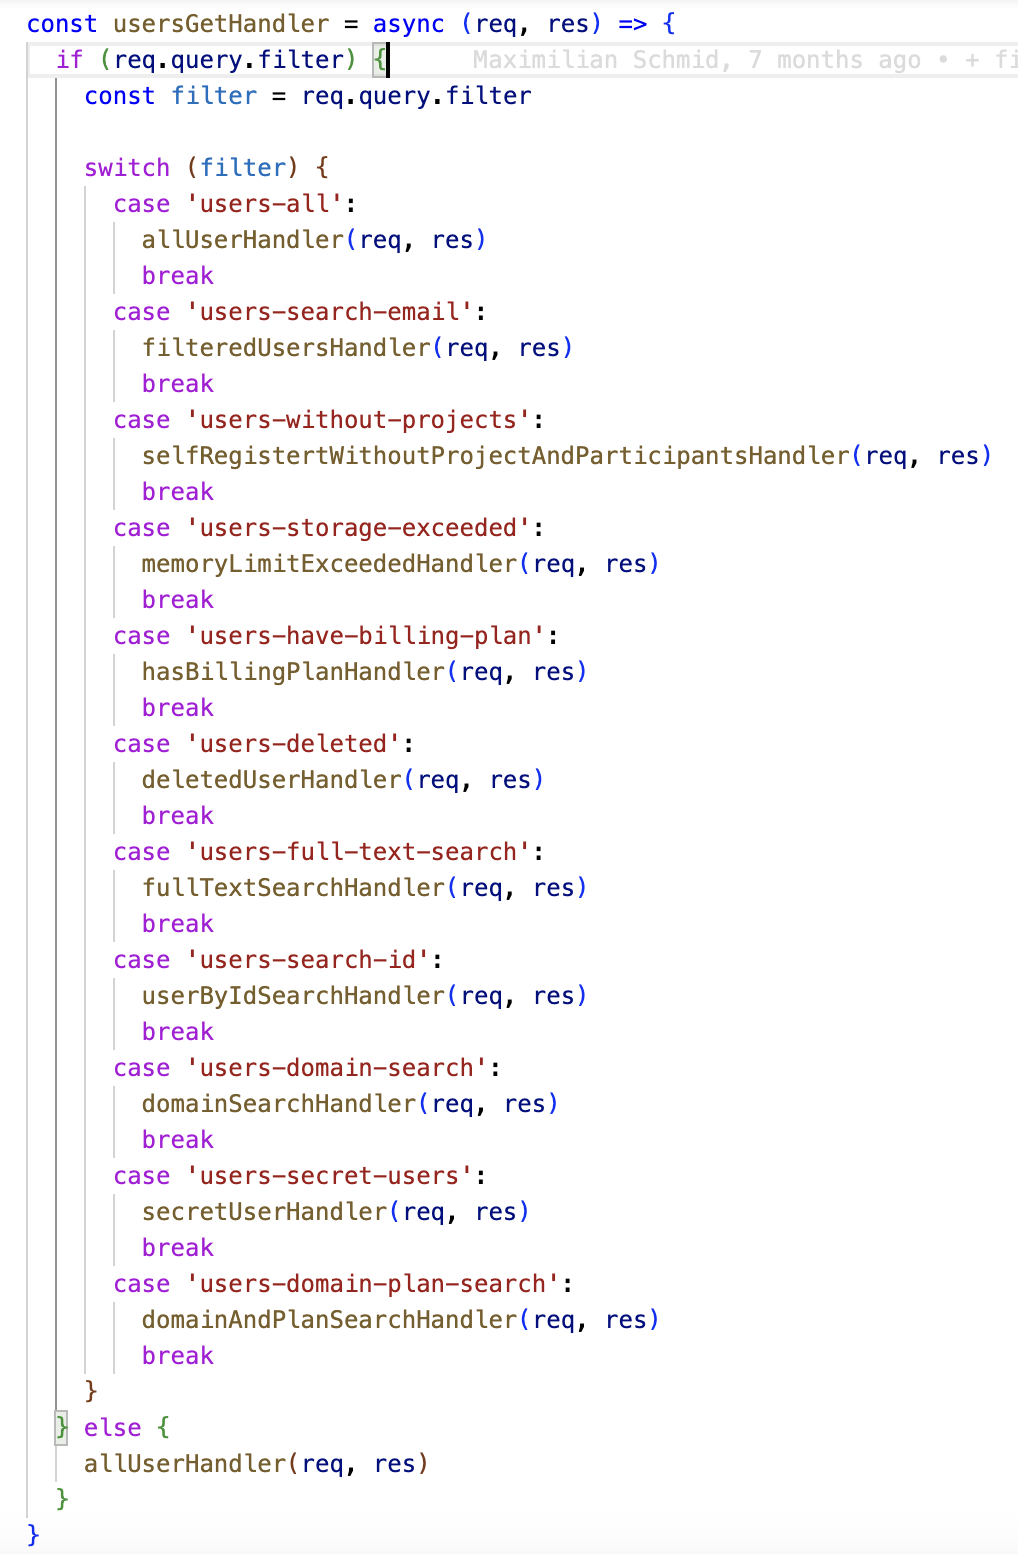
\includegraphics[width=0.6\textwidth]{pics/REST_API_Img.png}
    \caption{User-GET-Handler}
    \label{fig:enter-label}
\end{figure}

\subsection{Users}
\setauthor{Felix Arzt}
In diesem Endpunkt werden ausschließlich User Objekte an den Benutzer oder die Benutzerin zurück gegeben. Aufgrund von der Performance, werden bei allen Endpunkten nur die ersten 25 Objekte aus der Datenbank abgefragt und mit einem Button im Frontend, kann man die nachfolgenden 25 Benutzer nachladen. Folgende Endpunkte wurden dabei definiert und erledigen folgende Aufgaben:
\begin{itemize}
    \item \textbf{/users-all}
        \newline
        Bei diesem Endpunkt werden alle Benutzer aus der Datenbank zurückgeliefert. Es gibt die Option die Benutzer nach Login-Datum bzw. ...... zu sortieren.
    \item \textbf{/users-search-email}
        \newline
        Bei diesem Endpunkt werden ebenfalls standardmäßig alle Benutzer abgefragt, es gibt jedoch die Möglichkeit nach einer Email zu suchen. Dabei wird der eingegebene String ebenfalls als Übergabeparameter ans Backend übermittelt und dort überprüft, ob der String in der Email enthalten ist.
    \item \textbf{/users-without-project}
        \newline
        Bei diesem Endpunkt werden alle Benutzer zurückgegeben, welche sich selbst registriert haben (eigene Entity in Collection) und kein eigenes Projekt haben (ebenfalls eigene Entity in Collection).
    \item \textbf{/users-storage-exceeded}
        \newline
        Bei diesem Endpunkt werden alle Benutzer ermittelt, welche mit ihren eigenen Projekten den gebuchten Speicherplatz überschritten haben.
    \item \textbf{/users-have-billing-plan}
        \newline
        Bei diesem Endpunkt werden alle Benutzer zurückgegeben, welche noch keinen Zahlungsplan ausgewählt haben oder lediglich die Benutzer, welche einen Zahlungsplan ausgewählt haben. Diese Unterscheidung wird ebenfalls mit einem Übergabeparameter gelöst.
    \item \textbf{/users-deleted}
        \newline
        Grundsätzlich ist wichtig zu erwähnen, dass wenn ein Benutzer seinen Account eigenständig löscht, dieser nicht komplett aus der Datenbank entfernt wird, sondern eine Entity in der Collection auf true gesetzt wird. Deshalb werden bei diesem Endpunkt alle Benutzer angezeigt, welche ihren Account gelöscht haben.
    \item \textbf{/users-full-text-search}
        \newline
        Bei diesem Endpunkt werden alle Entitäten der Collection untersucht und auf einen Treffer geprüft und anschließend ans Frontend gesendet.
    \item \textbf{/users-search-id}
        \newline
        Bei diesem wird die ID ans Backend übergeben und der User mit dieser zurückgegeben.
    \item \textbf{/users-domain-search}
        \newline
        Dies ist ein eigener Endpunkt bei welchem nur auf die Domain der Email-Adresse geschaut wird und auf einen Treffer überprüft wird.
    \item \textbf{/users-secret-users}
        \newline
        Bei diesem Endpunkt werden alle Benutzer zurückgeliefert, welche keinen Zahlungsplan ausgewählt haben, jedoch trotzdem ein eigenes Projekt besitzen, in welchem in den letzten 30 Tagen ein Upload durchgeführt worden ist.
    \item \textbf{/users-domain-plan-search}
        \newline
        Bei diesem Endpunkt können alle Benutzer zurückgegeben werden, die keinen Zahlungsplan aktiviert haben und einen bestimmten Teil in der Email haben.
    \item \textbf{/changePlan/:id}
        \newline
        Bei diesem Endpunkt kann man den Zahlungsplans eines Benutzer auf none stellen.
    \item \textbf{/editPlan/:id}
        \newline
        Bei diesem Endpunkt kann man den Zahlungsplan individuell verändern. Man kann zum Beispiel den Speicherplatz verändern oder einen anderen vordefinierten Zahlungsplan auswählen.
\end{itemize}

\subsection{Projects}
\setauthor{Felix Arzt}
In diesem Endpunkt werden nur Projekt Objekte zurückgegeben, wie auch bei den User werden hier nur die ersten 25 Objekte geladen. Folgende Endpunkte wurden hier implementiert:
\begin{itemize}
    \item \textbf{projects-all}
        \newline
        Bei diesem Endpunkt werden alle Projekte abgerufen.
    \item \textbf{projects-deleted}
        \newline
        Wenn ein Projekt vom Benutzer gelöscht wird, wird es nicht aus der Datenbank gelöscht sondern lediglich das Field "trashed" auf true gesetzt. Bei diesem Endpunkt werden daher alle gelöschten Projekte zurückgegeben, bei welchem trashed = true ist.
    \item \textbf{projects-search-title}
        \newline
        Bei diesem Endpunkt werden defaultmäßig alle Projekte angezeigt, man kann allerdings nach dem Titel suchen. Dabei wird ein String ans Backend übergeben und dort überprüft, ob er in der Collection vorkommt.
    \item \textbf{projects-full-text-search}
        \newline
        Bei diesem Endpunkt wird jedes Field der Collection durchsucht und überprüft, ob der String darin vorkommt und anschließend zurückgegeben.
    \item \textbf{projects-search-id}
        \newline
        Bei diesem Endpunkt wird eine ID übergeben und das dazugehörige Projekt returned.
\end{itemize}

\section{CRUD Operations}
\setauthor{Nico Obermair}
Der Begriff CRUD steht für Create, Read, Update und Delete. Dies sind vier grundlegende Operationen in der Datenverarbeitung. Oft bilden diese Operationen die grundlegende Schnittstelle zwischen Andwendungen und Datenbanken.
\newline
\begin{figure}[h!]
    \centering
    
\includegraphics[width=0.8\textwidth]{pics/CRUD.jpeg}
    \caption{CRUD Operations}
    \label{fig:enter-label}
\end{figure}


 \subsection{Create}

 Bei der Create Operation geht es darum, neue Daten in die Datenbank zu persistieren. Es können beispielsweise neue Benutzer:innen oder Pläne angelegt werden.


 \subsection{Read}

 Die Read-Operation ergmöglicht es, vorhandene Daten aus der Datenbank auszulesen. Dies erfolgt in der Form von Abfragen, um Datensätze nach bestimmten Kritierien zu filtern, oder gegebenenfalls auch alle Datensätze abzurufen.

\begin{lstlisting}[caption=Read-Operation]
async function getProjectById (id) {
  if (!id) {
    throw new Error('ID must be provided')
  }
  const collection = planfredDbReadOnly.db.collection('projects')

  try {
    return collection.findOne({ _id: new ObjectId(id) })
  } catch (err) {
    throw new Error(err)
  }
}
\end{lstlisting}

Dieses Code Beispiel ist eine asynchrone Funktion names "getProjectById" welche ein Projekt anhand der ID aus der Datenbank ausliest.\newline
Zu Beginn wird überprüft, ob eine ID übergeben wurde. Falls nicht, wird mittels des "Early Return Pattern" sofort ein Fehler ausgelöst. Wenn die ID korrekt übergeben wurde, wird die entsprechende Collection, in diesem Fall "projects", in einer Variable gespeichert. Anschließend wird versucht, das entsprechende Projekt mit Hilfe eines Try-Catch-Statements abzurufen. Auch hier gilt wieder, sollte irgendwo in diesem Code Block ein Fehler vorkommen wird sofort ein Fehler ausgelöst.



\subsection{Update}

Die Update-Operation wird verwendet, um bereits bestehende Datensätze in der Datenbank zu verändern. Das können beispielsweise Anpassungen von Adressen in einer Kundendatenbank, oder Preisänderungen in einer Produktdatenbank sein. Ähnlich wie bei READ-Operationen können UPDATE-Operationen, abhängig von den ausgewählten Kriterien, auf sämtliche Datensätze, oder nur auf ausgewählte beschränkt werden.

Manche Big-Data-Systeme verzichten gänzlich auf die Integration der UPDATE-Operation und ermöglichen stattdessen ausschließlich eine CREATE-Operation in Verbindung mit einem Zeitstempel. Dabei wird bei jeder Aktualisierung eine neue Version der Zeile hinzugefügt.

\begin{lstlisting}[caption=Update-Operation]
try {
    const response = await fetch(`${config.planfredApiUrl}crm/projects/` + req.params.id, {
      method: 'PATCH',
      headers: {
        'Content-Type': 'application/json'
      },
      body: JSON.stringify(req.body)
    })
    const responseJSON = await response.json()
    return res.json(responseJSON)
  } catch (e) {
    console.error(e)
  }
\end{lstlisting}
\newpage
Dieses Code Beispiel verwendet die Node.js Fetch API. 

\begin{lstlisting}
    const response = await fetch(`${config.planfredApiUrl}crm/projects/` + req.params.id, {method: 'PATCH' })
\end{lstlisting}

In diesem Teil wird ein API-Aufruf mit fetch() durchgeführt, um die angegebene Ressource zu aktualisieren. Die URL für den API-Aufruf wird durch Verketten von config.planfredApiUrl, dem Teil der URL für die API, und req.params.id, dem Parameter aus der Anfrage, erstellt. Der API-Aufruf wird mit der Methode 'PATCH' ausgeführt, um eine partielle Aktualisierung der Ressource durchzuführen. Die Anfrage erfolgt asynchron, da "await" verwendet wird, um auf die Antwort zu warten.\newline

Im nächsten Teil werden die Headers gesetzt. In diesem Fall wird der "Content-Type" Header auf "application/json" gesetzt. Somit kann als Rückgabe Wert ein JSON Objekt zurückgegeben werden. Im Body wird der Inhalt der Anfrage festgehalten, hier wird JSON.stringify verwendet, um die Daten in ein JSON Format zu konvertieren, welches von der API erwartet wird.

\subsection{Delete}


Die DELETE-Operation erlaubt es den Nutzer:innen, Datensätze aus der Datenbank zu löschen. Bei einem endgültigen Löschen wird der Datensatz vollständig entfernt, während er beim vorläufigen Löschen markiert wird, aber an seinem aktuellen Ort bleibt.



In dieser Diplomarbeit wurden hauptsäclich READ und UPDATE-Operations verwendet. Die Syntax um ein Projekt zu löschen sieht wie folgt aus.

\begin{lstlisting}[caption=Delete-Operation]
    const project = await Projects.findById(req.params.id)

  try {
    project.trashed = req.body.value.new
    project.trashedDate = new Date()

    await project.save()

    res.json({ success: true })
  } catch (e) {
    next(e)
  }
\end{lstlisting}

Zu Beginn wird die Suche nach dem Projekt anhand der ID durchgeführt. Anschließend wird in einem Try-Catch-Statement versucht zwei Eigenschaften zu modifizieren. Zum einen wird das Attribut "project.trashed" angepasst, das vom Datentyp Boolean ist und daher entweder den Wert "true" oder "false" annehmen kann. Zusätzlich wird das Attribut "project.trashedDate" gesetzt, das vom Datentyp "Date" ist, um den exakten Zeitstempel zu dokumentieren, wann die Änderung am Projekt vorgenommen wurde.

Nachdem das Projekt erneut gespeichert wurde, wird bei erfolgreicher Ausführung aller Operationen eine Antwort über "res.json" gesendet, die einen Booleschen Wert zurückgibt, der "true" lautet.


Weiters wurden die Änderung des Speicherplatzes, sowie die Änderung des Abonnements nach dem selben Prinzip implementiert.
\cite{CRUD_Operations}

\subsection{Node.js Fetch API}
Die Fetch-API ist eine Programmierschnittstelle zur Abfrage von Netzwerkressourcen. Sie erleichtert das Senden von HTTP-Anfragen wie GET, POST usw.

Die Fetch-API unterstützt neue Standards wie Promise, was zu saubererem Code führt, der keine Rückrufe erfordert.

Die native Unterstützung für die Fetch-API ist in allen gängigen Browsern vorhanden. JavaScript-Entwickler verlassen sich für den serverseitigen Code auf das npm-Paket "node-fetch". Das Paket ist äußerst beliebt und wird jede Woche millionenfach heruntergeladen.

In dieser Diplomarbeit wurde die Fetch-API hauptsächlich für Updates verwendet. Diese Updates wurden nicht direkt in die Datenbank geschrieben, sondern zunächst an das Backend der Planfred-App gesendet und von dort aus in die Datenbank übertragen. Dies bietet einen erheblichen Sicherheitsvorteil. Dadurch benötigt das PlanfredCRM-Tool keinen Schreibzugriff auf die Produktionsdatenbank und ist somit sicherer.

\begin{figure}[h]
    \centering
    
\includegraphics[width=0.8\textwidth]{pics/fetch-api.png}
    \caption{Fetch API}
\end{figure}



\cite{Fetch_API}


\section{Authentification}
\setauthor{Nico Obermair}
Die Authentifizierung hat eine wesentliche Rolle im Rahmen dieser Diplomarbeit gespielt. Es war notwendig, eine Authentifizierung während des Anmeldevorgangs zu implementieren, um sicherzustellen, dass Benutzer für bestimmte API-Endpunkte spezifische Berechtigungen besitzen, um nicht nur Lesezugriff zu erhalten, sondern auch Änderungen vornehmen zu dürfen.


\subsection{JWT}
\setauthor{Nico Obermair}
JWT steht für "JSON Web Token" und repräsentiert einen offenen Standard (RFC 7519). Er ist zur Authentifizierung und Autorisierung gedacht, dieser Token kann sowohl vom Server als auch vom Client ausgelesen werden. Er kann verwendet werden um Daten sicher zwischen verschiedenen Anwendungen zu übermitteln. Durch die Signatur des JWT kann immer sichergestellt werden, dass nichts vom Inhalt manipuliert wurde.


\subsection{Wie ist ein JWT aufgebaut?}
Ein JWT ist grundlegend in drei Bereiche gegliedert:

\begin{itemize}
\item \textbf{Header}
\item \textbf{Payload}
\item \textbf{Signatur}
\end{itemize}

Es ist grundsätzlich ein einfacher Zeichenstring welcher in drei verschiedene Teile gegliedert wird, welche jeweils nur mit einem Punkt getrennt sind und mit Base64 kodiert sind. Ein Token lässt sich in folgender Form darstellen:

\begin{lstlisting}
Header.Payload.Signatur
\end{lstlisting}


\begin{figure}[h!]
    \centering
    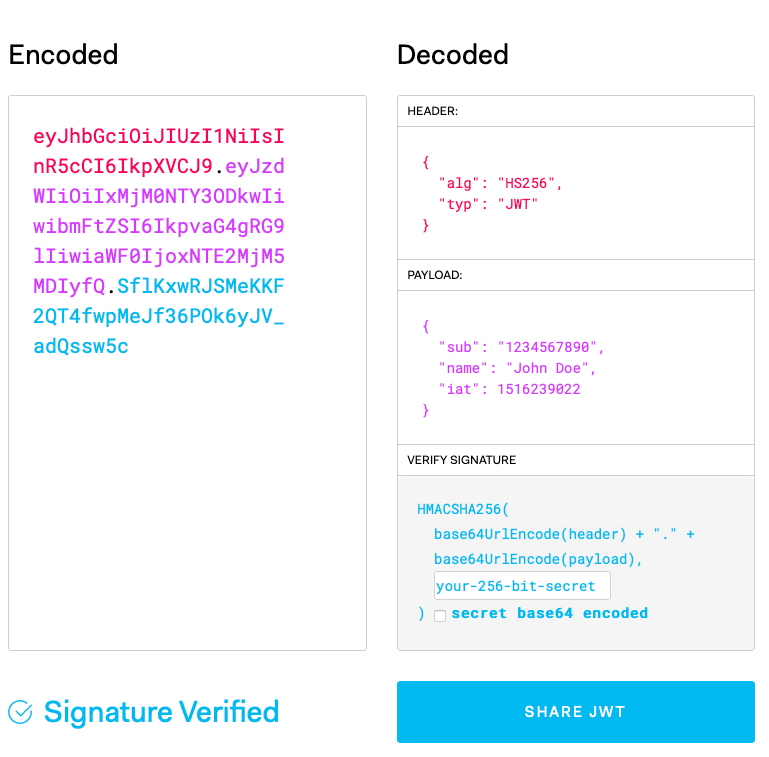
\includegraphics[width=0.6\textwidth]{pics/jwt.png}
    \caption{JSON Web Token}
    \label{fig:enter-label}
\end{figure}


\subsubsection{Header}

Der Header wird auch als JOSE (JSON Object Signing and Encryption) bezeichnet. In diesem sind ausschließlich Informationen über die Signierung und Verschlüsselung des JWT enthalten.


Typischerweise enthält die Struktur eines JWT-Headers eine Information über den Algorithmus, welcher zur Erstellung der Signatur verwendet wurde, sowie eine Definition, dass es sich um ein Json Web Token handelt. Dabei ist zu beachten, dass die Angabe des Typs optional ist, jedoch häufig auf "JWT" festgelegt wird. Dies ist besonders relevant für Anwendungen, die auch andere Typen, wie beispielsweise einen Access Token, akzeptieren, welcher jedoch in einer ähnlichen Datenstruktur vorliegt, um die verschiedenen Typen leicht voneinander unterscheiden zu können.

\begin{lstlisting}
{
  "alg": "HS256",
  "typ": "JWT"
}
\end{lstlisting}

\subsubsection{Payload}
Der zweite Part des JSON Web Token ist die Payload. Diese beinhaltet drei verschiedene Arten von Claims. 
Registrierte, Public und Private Claims

In den registrierten Claims sind zum Beispiel Sachen wie der Aussteller (iss) und die Ablaufzeit (exp) festgelegt.

Die Public Claims können nach Belieben definiert werden. Um jedoch Kollisionen zu vermeiden sollte der Name nicht gleich sein wie bei den registrierten Claims.

Die Privaten Claims sind individuelle Ansprüche, die erstellt wurden, um Informationen zwischen Parteien auszutauschen, die sich darauf einigen, sie zu verwenden, und die weder registrierte noch öffentliche Ansprüche sind.


\subsubsection{Signatur}

Der dritte Teil des JWT ist die Signatur diese ist in RFC 7515 definiert. Es kann sein das kein Algorithmus definiert wurde in diesem Fall entfällt die Signatur. Es gibt allerdings ganz seltene Fälle in denen dieses Verhalten erwünscht ist. 

\newline

Das zweite Verfahren wurde bereits erläutert. Dabei wird ein Algorithmus wie HS256 oder RS256 verwendet, um anhand der Daten einen eindeutigen Wert zu generieren und mögliche Manipulationen der Payload auszuschließen.

\newline

Das dritte Verfahren geht einen zusätzlichen Schritt weiter, indem es auf Verschlüsselung (JWE) setzt. Hier wird die Payload erneut mit einem privaten Schlüssel verschlüsselt und muss entsprechend entschlüsselt werden, um wieder im Klartext lesbar zu sein.

\subsection{Session vs. JSON Web Token}

\cite{JWT_1}

\cite{JWT_2"}

\cite{JWT_3}


\section{Postmark}
\setauthor{Nico Obermair}
Postmark ist ein Online-Service, welcher eine Email API zur Verfügung stellt. Diese API wurde in dieser Diplomarbeit verwendet um Mails an das Support Team zu versenden sobald eine Änderung in der Datenbank erfolgt ist. Das Hauptaugenmerk dieses Service liegt aber darin, dass die Emails auch wirklich in der Inbox ankommen und nicht im Spam landen. Diese Plattform implementiert bewährte Praktiken, um sicherzustellen, dass die Emails auch wirklich zuverlässig beim Empfänger ankommen. Dies funktioniert mit Funktionen wie Echtzeit-Protokollierung und Mechanismen zur Vermeidung von Spam.

Der Nachteil von Postmarkt liegt allerdings in den Kosten die dadurch verursacht wird. 10.000 Emails kosten monatlich 15 USD, bis zu einer Anzahl von 100 Emails pro Monat ist dieser Service kostenlos.

\begin{figure}[h!]
    \centering
    
\includegraphics[width=0.3\textwidth]{pics/postmark.png}
    \caption{Postmark}
    \label{fig:enter-label}
\end{figure}


\subsection{Mailversandfunktion}

In der folgenden Diplomarbeit wurde Postmarkt wie folgt verwendet


\begin{lstlisting}
// Send an email:
const client = new postmark.ServerClient(config.postmark.apikey)

async function mail (sub, body) {
  client.sendEmail({
    From: `${config.postmark.from}`,
    To: 'support@planfred.com',
    Subject: `${sub}`,
    HtmlBody: `${body}`
  })
}
\end{lstlisting}

Zuerst wird ein Client angelegt:
\begin{lstlisting}
new postmark.ServerClient(config.postmark.apikey)
\end{lstlisting}
In der Config ist der API-Key definiert welcher benötigt wird um Postmark verwenden zu können.

Die Funktion "client.sendEmail()" braucht einige Parameter:

\begin{itemize}
    \item \textbf{From}
        \newline
        Hier wird die Absender E-Mail Adresse definiert. Diese kann beliebig gewählt werden.
    \item \textbf{To}
        \newline
        In diesem Parameter wird die Empfänger E-Mail definiert.
    \item \textbf{Subject}
        \newline
        Im Subject wird der Betreff des E-Mails definiert.
    \item \textbf{HtmlBody}
        \newline
        Im HtmlBody wird der Inhalt in die E-Mail geschrieben. Dieser kann als HTML Code geschrieben werden.
\end{itemize}


Weiteres können noch andere Properties wie zum Beispiel Header, TextBody, oder Cc gesetzt werden:

\begin{lstlisting}
{
  "From": "sender@example.com",
  "To": "receiver@example.com",
  "Cc": "copied@example.com",
  "Bcc": "blank-copied@example.com",
  "Subject": "Test",
  "Tag": "Invitation",
  "HtmlBody": "<b>Hello</b>",
  "TextBody": "Hello",
  "ReplyTo": "reply@example.com",
  "Metadata": {
      "Color":"blue",
      "Client-Id":"12345"
  },
  "Headers": [
    {
      "Name": "CUSTOM-HEADER",
      "Value": "value"
    }
  ],
  "TrackOpens": true,
  "TrackLinks": "HtmlOnly",
  "MessageStream": "outbound"
}
\end{lstlisting}







Mit der "mail" Funktion wird also eine Email versendet diese funktioniert einfach nur durch 
\begin{lstlisting}
client.sendEmail({})
\end{lstlisting}


\section{Datenbankverbindung}
\setauthor{Felix Arzt}
Content